% !TEX root = ../main.tex
\section{Introduction}
In statistical physics, building a model corresponding to a physical system is useful: comparing how the model's predictions differ from experiment can be used to understand how a system behaves. For computing properties corresponding to a model's behavior, the normalization constant of the model's Boltzmann distribution in \Cref{eq:boltzmann} is a central quantity. The partition function can be used to derive properties of physics models that can be measured in experimental realizations, such as specific heat or magnetization. Such properties of models can be compared to experimental values, which can inform how a model might be improved to better mirror reality. But the partition function is intractable for many probabilistic models of interest, as described in \Cref{ch:background}.

One workaround to the problem of an intractable partition function is to use an approximate inference algorithm such as \gls{mcmc}. \gls{mcmc} relies on sampling likely configurations of a system and does not require calculating the partition function. In theory, these samples will be draws from the probability model of interest~\citep{metropolis1953equation,andrieu2003an-introduction}. For example, samples from the Boltzmann distribution can be used to approximate physical quantities derived from the probability model, such as specific heat.

However, with limited computation \gls{mcmc} has limitations. This method requires practitioners to use convergence diagnostics~\citep{brooks1998general} to assess whether samples from the algorithm are independent. Scalable \gls{mcmc} requires careful consideration. While some scalable versions of \gls{mcmc} have been developed~\citep{neal2011mcmc,welling2011bayesian}, they are biased samplers that may not have guaranteed convergence to samples from the probability model of interest. This is similar to how in \gls{vi} performance must often be assessed empirically. But in comparison to \gls{vi}, unless a model-specific algorithm has been developed~\citep{wolff1989comparison}, generic \gls{mcmc} methods do not readily scale to large numbers of random variables.
% - describe the contributions of our paper: (1) show that
% gibbs-bogoliubov-feynman inequality is equivalent to variational inference.
% (1) show how the reinforcement learning approach of wu (2019) is more
% naturally expressed in terms of variational inference. (2) show that a modern
% tool of variational inference, HVMs, is useful and improves on wu (2019) by
% scaling to larger system sizes.

In \Cref{ch:background} we showed that the machine learning framework of \gls{vi} is equivalent to the \acrlong{gbf} variational principle. This has allowed practitioners to study statistical physics models using many variational approximations, including \glspl{van}. As an example of a variational method enabled by \gls{vi}, we study \glspl{hvm} as approximations to the Boltzmann distribution of statistical physics models. We find that \glspl{hvm} scale to larger systems sizes than \glspl{van} in Sherrington-Kirkpatrick and Ising models. Testing the feasibility of \gls{vi} methods in statistical physics is a twofold opportunity. Statistical physics problems might serve as benchmarks for \gls{vi}, and using \gls{vi} for these problems can lead to improved computational methods in statistical physics. % and where exact solutions ar eknown?
\paragraph{Related Work.} The \gls{gbf} variational principle has been used to study Markov random fields~\citep{jun-zhang1996the-application} and the connection between variational inference and statistical physics has been well-documented~\citep{blei2017variational,hoffman2013stochastic,mackay2003information}. But this equivalence between \gls{vi} and the \gls{gbf} inequality might serve as an introduction to \gls{vi} for physicists. \citet{wu2019solving} implicitly use \gls{vi}, by developing \glspl{van} and a reinforcement learning policy gradient algorithm (however, \gls{vi} is not mentioned). Further, for a system of size $L$, autoregressive neural networks require $\cO(L^2)$ forward passes to sample a system configuration, making \glspl{van} intractable in larger systems. The use of \glspl{hvm} can be advantageous for statistical physics as these models can sample from a system in $\cO(L)$ time and yield results for larger systems.

\paragraph{Variational Inference.}
\gls{vi} is equivalent to the \gls{gbf} variational principle and requires similar choices of a practitioner. The variational family $q(\mbz; \mbnu)$ to approximate a model must be chosen, in addition to a method to maximize the variational lower bound in \Cref{eq:llbo}.

The \gls{vi} literature provides several choices of variational family, such as a mean field, factorized variational distribution with independent latent variables. Another choice of variational family is the Bethe approximation, which constrains the variational distribution to the polytope of mean parameters that captures correlations between any two latent variables~\citep{wainwright2008graphical}. Some machine learning research focuses on developing variational approximations that capture correlations between latent variables~\citep{hoffman2015stochastic,kingma2016improved,maaloe2016auxiliary,wu2019solving}. An example of a variational family that can model correlations between latent variables is the \gls{van} family~\citep{wu2019solving}, which uses autoregressive neural networks to parameterize the variational distribution ${q(\mbz_i \mid \mbz_1, \ldots, \mbz_{i-1})}$. We explore the \gls{hvm} class of variational approximations~\citep{ranganath2018black}.

The second choice required to employ \gls{vi} is how to optimize the variational lower bound in \Cref{eq:llbo}. The choice of variational family can limit the available optimization techniques. For a simple variational family like the mean field approximation, it may be possible to analytically evaluate the expectations in \Cref{eq:llbo}. Then derivatives of the variational bound with respect to the variational parameters $\mbnu$ and manual calculation can maximize the lower bound, as derived in \Cref{sec:ising-mean-field}. If more expressive variational families are used (e.g. \gls{van}s with thousands or millions of variational parameters), the analytic approach is infeasible. Stochastic optimization and automatic differentiation software have been used to develop several approaches to computing gradients of the variational lower bound, such as \acrlong{bbvi}~\citep{ranganath2018black,mohamed2019monte}.
% !TEX root = ../../main.tex
\newcommand{\mywidtht}{0.25\textheight}
\newcommand{\figwidtht}{0.3\textheight}
\begin{figure}[t]
  \centering
  % adjust margin to center captions
  \captionsetup[subfigure]{justification=centering,margin={0cm,0cm},oneside}
  \hfill%\hspace{\mywidtht}%
  \begin{subfigure}[b]{\figwidtht}
    \centering
    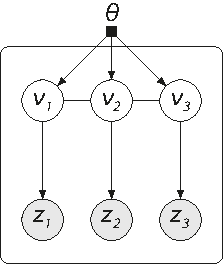
\includegraphics[width=\mywidtht]{ch-hvm/fig/hierarchical-variational-model.pdf}
    % \caption{\Acrlong{hvm}}%
    \label{fig:hvm-graphical-model}%
  \end{subfigure}
  \hspace*{\fill}%
  \begin{subfigure}[b]{\figwidtht}
    \centering
    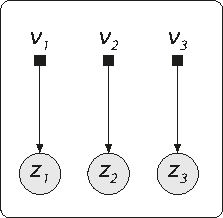
\includegraphics[width=\mywidtht]{ch-hvm/fig/mean-field-graphical-model.pdf}
    % \caption{Mean-field variational family}%
    \label{fig:mean field-graphical-model}%
  \end{subfigure}
  \hspace*{\fill}%
  % \vspace{-0.5cm}
  \caption[\textsc{hvm} and mean field approximation graphical models]{\textbf{\Acrlongpl{hvm} (\glspl{hvm}, left) capture dependencies between latent variables, compared to the mean field variational family with independent variables (right).}}
  \label{fig:graphical-model}
\end{figure}

The choice of variational family $q(\mbz; \mbnu)$ and optimization method for maximizing the variational lower bound leads to a trade-off intrinsic to \gls{vi}. Simple variational approximations such as the mean field family may be computationally feasible but inaccurate. The cost of increased accuracy, say by using a structured variational approximation, is increased computation. We illustrate the use of \gls{vi} in statistical physics by comparing two choices of variational approximation, \glspl{hvm}~\citep{ranganath2018black} and \glspl{van}~\citep{wu2019solving}. Many other variational approximations can be explored in future work.
